\documentclass[twoside]{article}
\usepackage[a4paper]{geometry}
\geometry{verbose,tmargin=2.5cm,bmargin=2cm,lmargin=2cm,rmargin=2cm}
\usepackage{fancyhdr}
\pagestyle{fancy}

% nastavení pisma a~češtiny
\usepackage{lmodern}
\usepackage[T1]{fontenc}
\usepackage[utf8]{inputenc}
\usepackage[czech]{babel}

% odkazy
\usepackage{url}

\usepackage{float}
% vícesloupcové tabulky
\usepackage{multirow}
\usepackage{listings}
\usepackage{amssymb}
\usepackage{gensymb}
\usepackage{bbold}
\usepackage{amsmath}
\usepackage{siunitx}
\usepackage{mathtools}
\usepackage{commath}

% vnořené popisky obrázků
\usepackage{subcaption}

% automatická konverze EPS 
\usepackage{graphicx} 
\usepackage{epstopdf}
\epstopdfsetup{update}

\graphicspath{{./images}}

% odkazy a~záložky
\usepackage[unicode=true, bookmarks=true,bookmarksnumbered=true,
bookmarksopen=false, breaklinks=false,pdfborder={0 0 0},
pdfpagemode=UseNone,backref=false,colorlinks=true] {hyperref}

% Poznámky při překladu
\usepackage{xkeyval}	% Inline todonotes
\usepackage[textsize = footnotesize]{todonotes}
\presetkeys{todonotes}{inline}{}

%https://tex.stackexchange.com/questions/2783/bold-calligraphic-typeface
\DeclareMathAlphabet\mathbfcal{OMS}{cmsy}{b}{n}

% enumerate zacina s pismenem
\renewcommand{\theenumi}{\alph{enumi}}

% smaz aktualni page layout
\fancyhf{}
% zahlavi
\usepackage{titling}
\fancyhf[HC]{\thetitle}
\fancyhf[HLE,HRO]{\theauthor}
\fancyhf[HRE,HLO]{\today}
 %zapati
\fancyhf[FLE,FRO]{\thepage}

% údaje o autorovi
\title{Automatické řízení: DÚ 10 -- Diskrétní řízení}
\author{Vojtěch Michal}
\date{\today}

\begin{document}

\maketitle

Jsem narozen 18. února 2000. Proto volím $a = 8$, $b = 2$, odtud dále $c = \frac{a+b-2}{4} + 4 = 6$.

Zadaná soustava má přenos 
\begin{equation}
	G(s) = \frac{s+9}{s^2+5s-6}.
\end{equation}

Pro Vaši soustavu navrhněte diskrétní regulátor pro vzorkovací periodu $h = 0.05$ \si{\second}. Vstupní signál $u$ do
soustavy je omezen na $-1.5 \le u \le 1.5$. Požadavky na regulaci:
\begin{enumerate}
	\item Regulátor pracuje s výstupem systému, nezná všechny jeho stavy.
	\item Regulátor zajistí nulovou ustálenou regulační odchylku při odezvě na skok.
	\item Maximální překmit odezvy na skok je $OS = 30$ \%.
	\item Doba ustálení na $\pm 5$\% od požadované hodnoty odezvy na skok je nejvýše $3$ \si{\second}.
	\item Pokud použijete integrační složku, musí být implementován anti-windup.
\end{enumerate}

\section{Výběr metody regulace}

Po diskretizaci soustavy Tustinovou metodou s krokem $h$ získám diskrétní přenos druhého řádu
\begin{equation}
	G(z) = \frac{  0.02731 z^2 + 0.01003 z - 0.01728}{  z^2 - 1.79 z + 0.777},
\end{equation}
jehož odezva na jednotkový skok je vykreslena na obrázku \ref{fig:porovnani}. Diskretizace je zřejmě věrná,
oba přenosy $G(s)$ i $G(z)$ jsou nestabilní a divergují do nekonečna. Na základě požadavků zadavatele na dynamiku
uzavřené zpětnovazební smyčky je možné rovnou vyřadit návrh stavové zpětné vazby. Dále protože je požadováno
asymptotické sledování skoku, jsou vhodnými kandidáty regulátor se dvěma stupni volnosti a nebo regulátor z rodiny PID.

\begin{figure}[htbp]
	\centering
	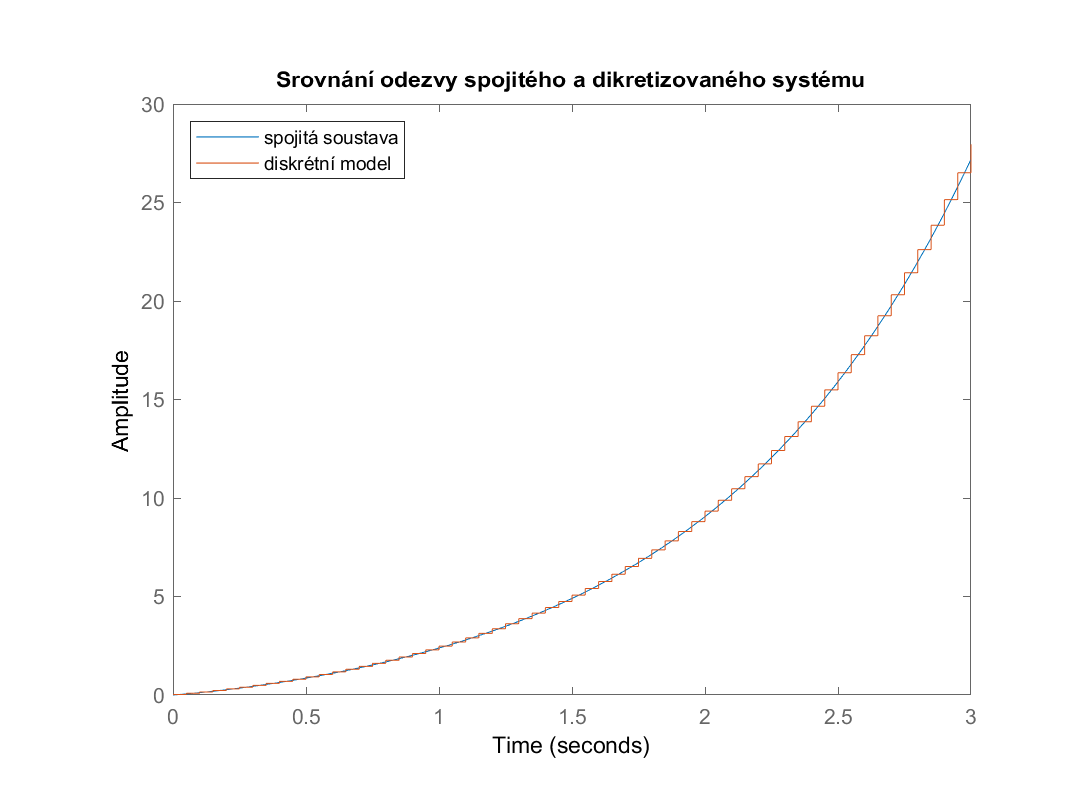
\includegraphics[width=.8\linewidth]{porovnani_nestabilni.eps}
	\caption{Ověření věrohodnosti diskretizace Tustinovou metodou}
	\label{fig:porovnani}
\end{figure}

Protože 2DOF není v tomto případě nezbytný, zatímco PID je dostačující (regulovaná soustava je druhého řádu), volím jej.
Pro začátek návrhu vynechám derivační složku a navrhuji jen diskrétní PI regulátor (též nazýván PS regulátor).
Opět ji uvážím jen kdyby nebylo možné systém snadno stabilizovat.

Pomocí nástroje Matlabu \textit{PIDTuner} pro diskrétní přenosou funkci $G(z)$ ladím regulátor pro splnění zadaných
požadavků v časové oblasti. Požadavek na $OS$ lze volbou agresivního regulátoru splnit velice rychle (doba ustálení pod 1 \si{\second}),
ovšem takováto regulace by vyžadovala velkou hodnotu akčního zásahu. S vědomím, že akční zásah do soustavy je saturován, se snažím
maximálně zpomalit regulaci, což zajistí pozvolnější přeběhy a tedy menší absolutní hodnoty akčního zásahu $u(z)$, jež nebudou trpět na saturaci. 


Výstupem je paralelní PS regulátor
\begin{equation}
	C(z) = \underbrace{4.8}_{=K_\text{P}} + \underbrace{4.83}_{=K_\text{I}} \frac{h}{z-1},
\end{equation}
jehož zapojení do zpětné vazby s dikrétní soustavou vede na skokovou odezvu vykreslenou na obrázku \ref{fig:stabilizace}.

\begin{figure}[htbp]
	\centering
	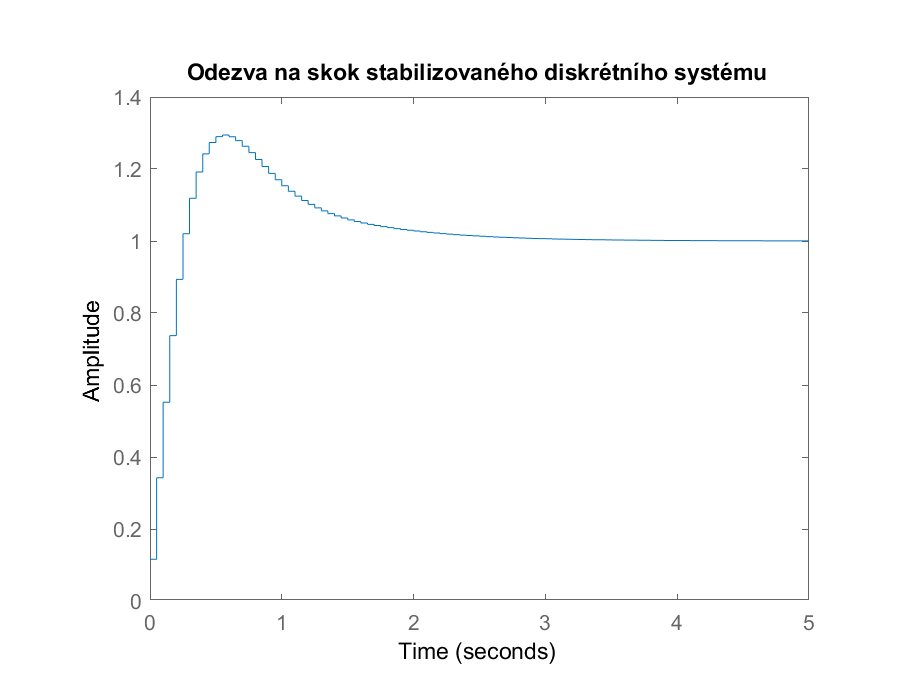
\includegraphics[width=.6\linewidth]{stabilizovany_diskretni.eps}
	\caption{Diskrétní systém po stabilizaci zpětnou vazbou}
	\label{fig:stabilizace}
\end{figure}

Je patrno, že regulátor je stabilizující alespoň pro diskrétní náhradu soustavy a že jsou splněny požadavky na regulaci.
Do přiloženého .m souboru je regulátor implementován následujícím blokem kódu

\begin{lstlisting}
    %constants of the regulator:
    Kp = 4.8; Ki = 4.83;
    
    %compute one iteration of the controller
    error = r(k) - y(k); %error term (input for the regulator)
    integral = integral + Ts * Ki * error;
    u(k) = Kp*error + integral;
    
    if abs(u(k)) > u_sat
       integral = 0; %integral anti-windup
    end
\end{lstlisting}

Simulace provedená skriptem potvrzuje splnění požadavků na dynamiku zpětnovazební smyčky.
Dosažený překmit je 19.4 \%, doba ustálení je 1.4 \si{\second}.

\begin{figure}[htbp]
	\centering
	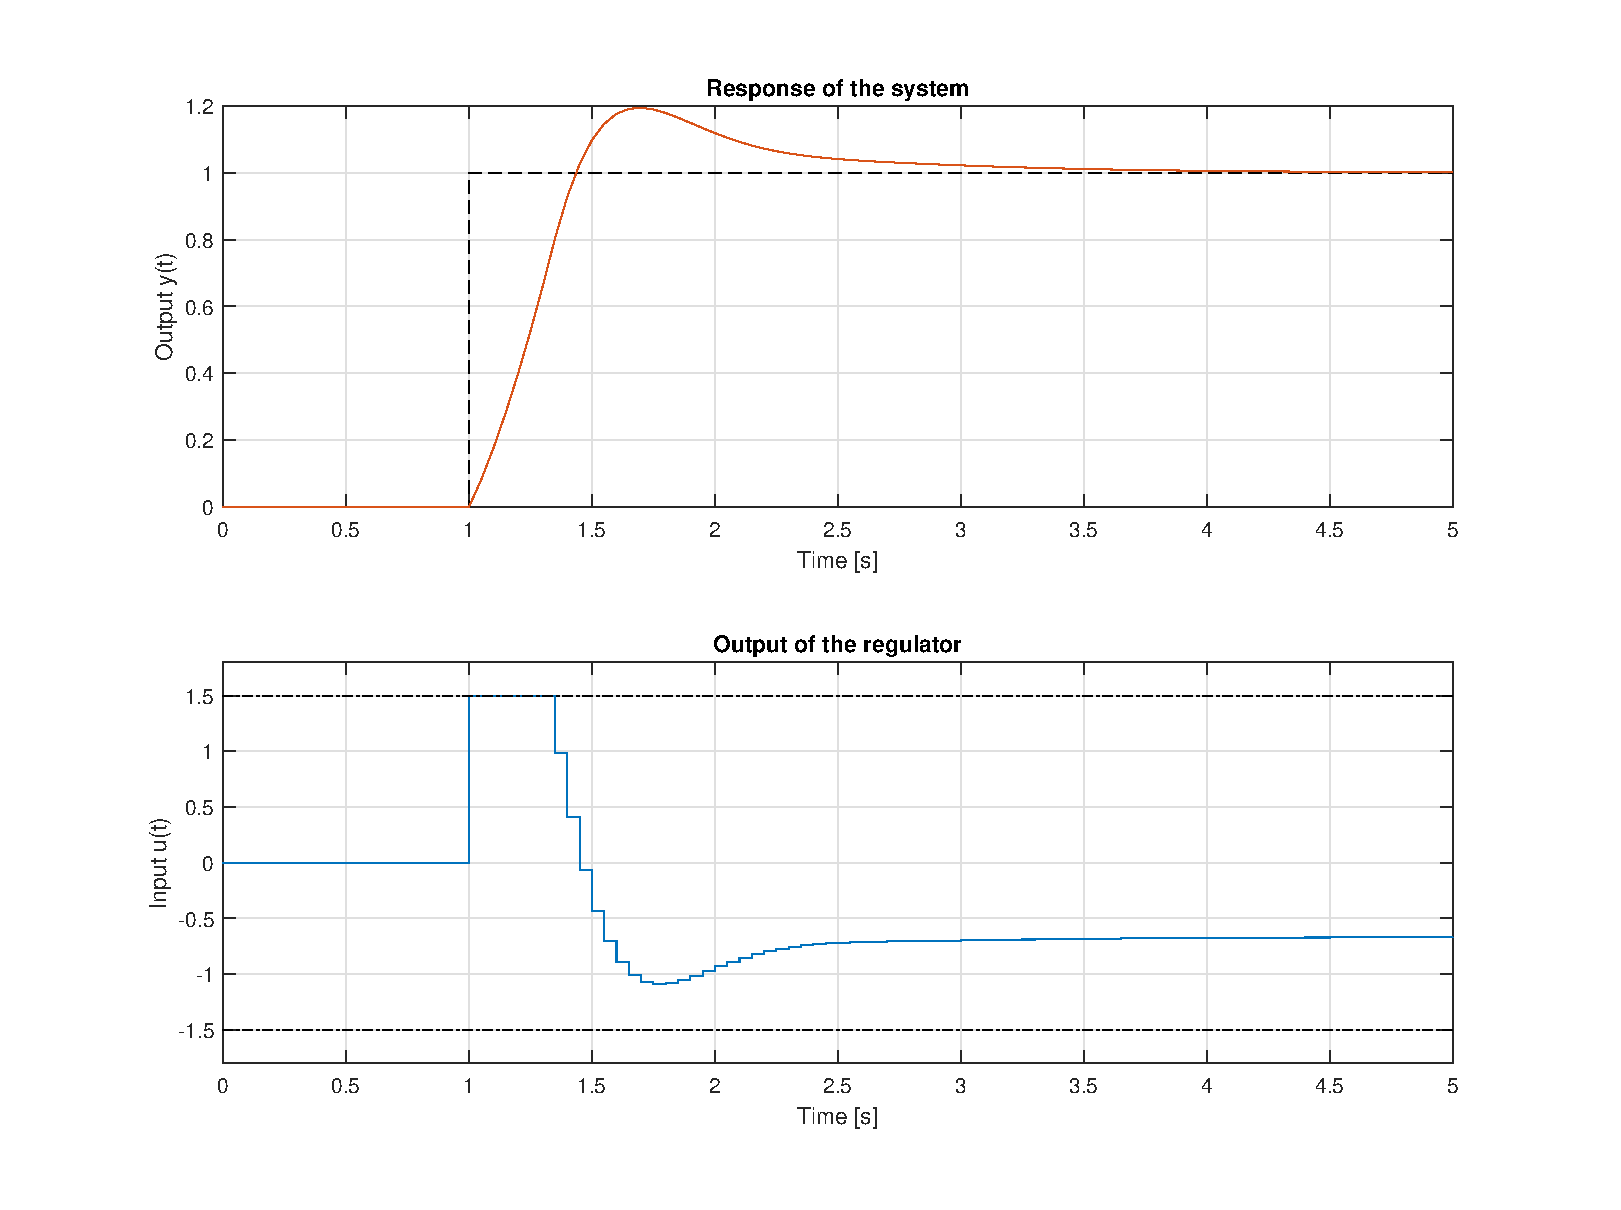
\includegraphics[width=.6\linewidth]{odezva_spojity.eps}
	\caption{Průběh signálů v uzavřené zpětnovazební smyčce}
	\label{fig:vysledek}
\end{figure}



\begin{thebibliography}{9}

	\bibitem{motivace}
		Motivační hudba, \emph{Kirby dream land theme song} \url{https://www.youtube.com/watch?v=3CS93CdMv_E}
	
	\end{thebibliography}

\end{document}

